\documentclass[reqno, a4paper]{amsart}
\author{J. Púček, L. Košárková, M. Fuksa}
\usepackage{amsmath}
\usepackage{amssymb}
\usepackage{amsthm}

\usepackage[scale=0.9]{geometry}
\usepackage{mathbbol}

\usepackage[utf8]{inputenc}
\usepackage[czech]{babel}

\usepackage{subfig}
\usepackage{graphicx}
\usepackage{multicol}
\usepackage[font=small,labelfont=bf]{caption}
\usepackage{graphicx,wrapfig}

%\makeatletter
% \@ifpackageloaded{tensor}% tensor is a package for a better typesetting of tensors
% {
% \renewcommand{\tnsr@Aux}[3][]{%
% \mathpalette{\tnsr@Plt{#1}{#3}}{\mathrm #2}%
% \tnsr@Wrn
% }%\tnsr@Aux
% }{%
% \relax%
% }
% \makeatother


% operators
\DeclareMathOperator{\divergence}{div}
\DeclareMathOperator{\Divergence}{Div}
\DeclareMathOperator{\gradient}{grad}
\DeclareMathOperator{\Gradient}{Grad}
\DeclareMathOperator{\rot}{rot}
\DeclareMathOperator{\Asym}{Asym}
\DeclareMathOperator{\Sym}{Sym}
\DeclareMathOperator{\Tr}{Tr}
\DeclareMathOperator{\signum}{sign}
\DeclareMathOperator{\supp}{supp}
\DeclareMathOperator{\cof}{cof} % cofactor
\DeclareMathOperator{\residue}{res}
\DeclareMathOperator{\ad}{ad} % adjoint ad_X (Y) = [X,Y]  
\DeclareMathOperator{\distanceop}{dist} % distance in a metric space

% Kernel, range, rank
\DeclareMathOperator{\kernelop}{{\mathcal N}}
\DeclareMathOperator{\rangeop}{{\mathcal R}}
\DeclareMathOperator{\rankop}{rank}

% jump
\newcommand{\jumpdis}[1]{\ensuremath{\left\lsem #1 \right\rsem}} % difference between function values at the point of jump discontinuity

% hyperbolic functions
\DeclareMathOperator{\arcsinh}{arcsinh}
\DeclareMathOperator{\arccosh}{arccosh}
\DeclareMathOperator{\arctanh}{arctanh}
\DeclareMathOperator{\arccoth}{arccoth}

% invariants of second order tensor
\DeclareMathOperator{\invariantI}{I_1}
\DeclareMathOperator{\invariantII}{I_2}
\DeclareMathOperator{\invariantIII}{I_3}

% big o
\newcommand{\bigo}[1]{\ensuremath{O\left(#1 \right)}}
\newcommand{\smallo}[1]{\ensuremath{o\left(#1 \right)}}

% exponential
\newcommand{\exponential}[1]{\ensuremath{{\mathrm e}^{#1}}}

% imaginary unit
\newcommand{\iunit}{\ensuremath{\mathrm{i}}}


% real and imaginary part
\newcommand{\realp}{\mathrm{real}}
\newcommand{\imagp}{\mathrm{imag}}

%\newcommand{\Real}{\Re}
%\newcommand{\Imag}{\Im}
\providecommand{\Real}{\Re}
\providecommand{\Imag}{\Im}

% predicates
\newcommand{\charac}{\ensuremath{\mathrm{char}}} % characteristic quantity such as length scale, etc.
\newcommand{\reference}{\mathrm{ref}}
\newcommand{\crit}{\mathrm{crit}}
\newcommand{\bydefinition}{\mathrm{def}}
\newcommand{\traceless}[1]{{#1}_{\delta}}

% dimensionless variables and functions
\newcommand{\dimless}[1]{#1^\star}

% derivatives
\newcommand{\diff}{\mathrm{d}}
\newcommand{\Diff}[1][]{\mathrm{D}_{#1}} % For Frechet and Gateaux derivative
\newcommand{\hDiff}[2][]{\mathrm{D}^{#1}_{#2}} % Higher order Frechet and Gateaux derivative

% inexact differential
\newcommand{\dbar}{{\mathchar'26\mkern-12mu \diff}}
\newcommand{\idiff}{\dbar}

% body
\newcommand{\body}{{\mathcal B}}

% vectors and tensors
\renewcommand{\vec}[1]{\ensuremath{\mathbf{#1}}}
\newcommand{\greekvec}[1]{\ensuremath{\boldsymbol{#1}}}
\makeatletter
\@ifpackageloaded{bm}% 
{\renewcommand{\vec}[1]{\ensuremath{\bm{#1}}}%
\renewcommand{\greekvec}[1]{\ensuremath{\bm{#1}}}%
}{%
\relax% do nothing
}
\makeatother
\newcommand{\tensorq}[1]{\ensuremath{\mathbb{#1}}}      % tensorial quantity
\newcommand{\tensorc}[1]{\ensuremath{\mathrm{#1}}}      % tensorial quantity components  

\newcommand{\conjugate}[1]{#1^\star}
\newcommand{\transpose}[1]{#1^\top}
\newcommand{\transposei}[1]{#1^{-\top}}
\newcommand{\inverse}[1]{#1^{-1}}

% Identity matrix and zero matrix
\newcommand{\identity}{\ensuremath{\tensorq{I}}} % identity
\newcommand{\tensorzero}{{\mathbb{O}}} % zero tensor

% Cauchy stress
\newcommand{\cstress}{\tensorq{T}}
\newcommand{\cstressc}{\tensorc{T}}

% Cauchy stress, thermodynamically determined part
%\DeclareMathSymbol{\robustrho}{\mathord}{letters}{"1A} % If I want to write \fid{\thcstressrho} it sometimes happes that the greek letters in subscript get crippled, this happens expecially in MDPI class. This tirck protects \rho. It would work also for other greek letters, the codes are given in  fontdef.dtx
\newcommand{\thcstress}{\ensuremath{\cstress_{\mathrm{th}}}} 
%\newcommand{\thcstressrho}{\ensuremath{\cstress_{\mathrm{th},\, \robustrho}}} % thermodynamically determined part divided by rho
\newcommand{\thcstressrho}{\ensuremath{\cstress_{\mathrm{th},\, \mathnormal{\rho}}}} % thermodynamically determined part divided by rho
\newcommand{\tracelessthcstress}{\traceless{\left(\thcstress\right)}} % traceless part
\newcommand{\tracelessthcstressrho}{\traceless{\left(\cstress_{\mathrm{th},\, \rho}\right)}} % traceless part divided by rho

% Extra stress tensor
\newcommand{\ecstress}{\tensorq{S}}
\newcommand{\ecstressc}{\tensorc{S}}

% First Piola stress tensor
\newcommand{\fpstress}{\tensorq{T}_{\mathrm{R}}}
\newcommand{\fpstressc}{\tensorc{T}_{\mathrm R}}

% Second Piola--Kirchhoff stress tensor
\newcommand{\spstress}{\tensorq{S}_{\mathrm{R}}}
\newcommand{\spstressc}{\ensuremath{{{\mathrm S}_{\mathrm R}}}}

% Couple stress tensor
\newcommand{\couplestress}{\tensorq{M}}
\newcommand{\couplestressc}{\tensorc{M}}

% deformation, deformation gradient
\newcommand{\deformation}{\greekvec{\chi}}
\newcommand{\deformationc}{\tensorc{\chi}}

\newcommand{\fgrad}{\tensorq{F}}
\newcommand{\fgradc}{\tensorc{F}}
\newcommand{\fgradrel}[3][]{\fgrad^{#1}_{#2}\left(#3\right)}

% determinant of deformation gradient, Jacobian
\newcommand{\detfgrad}{J}

% displacement
\newcommand{\displacement}{\vec{U}}
\newcommand{\displacementc}{\tensorc{U}}

% right Cauchy-Green tensor
\newcommand{\rcg}{\tensorq{C}}
\newcommand{\rcgc}{\tensorc{C}}        
\newcommand{\rcgrel}[3][]{\rcg^{#1}_{#2}\left(#3\right)}

% left Cauchy-Green tensor
\newcommand{\lcg}{\tensorq{B}}
\newcommand{\lcgc}{\tensorc{B}}        
\newcommand{\lcgrel}[3][]{\lcg^{#1}_{#2}\left(#3\right)}
\newcommand{\lcgb}{\overline{\lcg}} % rescaled left Cauchy--Green tensor, theory of slightly compressible materials
\newcommand{\lcgbc}{\overline{\lcgc}} % rescaled left Cauchy--Green tensor, theory of slightly compressible materials, components


%\newcommand{\piolastrain}{\tensorq{b}} % Piola deformation tensor (inverse of right Cauchy--Green)
%\newcommand{\fingerstrain}{\tensorq{c}} % Finger deformation tensor (inverse of left Cauchy--Green)

% rotation
\newcommand{\rotation}{\tensorq{R}}
\newcommand{\rotationrel}[3][]{\rotation^{#1}_{#2}\left(#3\right)}

% stretch
\newcommand{\stretchu}{\tensorq{U}}
\newcommand{\stretchurel}[3][]{\stretchu^{#1}_{#2}\left(#3\right)}
\newcommand{\stretchv}{\tensorq{V}}
\newcommand{\stretchvrel}[3][]{\stretchv^{#1}_{#2}\left(#3\right)}

% linearized strain (symmetric part of displacement gradient), skew-symmetric part of displacement gradient
\makeatletter
\@ifpackageloaded{bm}% 
{%
\newcommand{\linstrain}{\bbespilon} %requires \usepackage[bbgreekl]{mathbbol}
% YES, the spelling is wrong, but this is how it is coded in the package
}{%
\newcommand{\linstrain}{\tensorq{\varepsilon}}
}

\@ifpackageloaded{bm}%
{%
\newcommand{\skewdgradient}{\bbomega} 
}{%
\newcommand{\skewdgradient}{\tensorq{\omega}}
}

\@ifpackageloaded{bm}%
{%
\newcommand{\linstress}{\bbtau} % stress in linearised elasticity
}{%
\newcommand{\linstress}{\tensorq{\tau}}
}
\makeatother

\newcommand{\linstrainc}{\mathrm{\varepsilon}}
\newcommand{\linstressc}{\mathrm{\tau}}
\newcommand{\skewdgradientc}{\mathrm{\omega}}

% Lagrangean and Eulerian strain
\newcommand{\lstrain}{\tensorq{E}} % Green--Saint-Venant strain
\newcommand{\lstrainc}{\tensorc{E}} % Green--Saint-Venant strain, components
\newcommand{\estrain}{\tensorq{e}} % Euler--Almansi strain, components
\newcommand{\estrainc}{\tensorc{e}} % Euler--Almansi strain, components

% Hencky strain
\newcommand{\henckystrain}{\tensorq{H}} % Hencky strain
\newcommand{\henckystrainc}{\tensorc{H}} % Hencky strain, components

\newcommand{\devhencky}{\overline{\tensorq{H}}} % Hencky strain, deviatoric part via deviatoric deformation
\newcommand{\devhenckyc}{\overline{\tensorc{H}}} % Hencky strain, deviatoric part via deviatoric deformation, components


% Rivlin-Ericksen tensor
\newcommand{\rivlin}{{\tensorq{A}}}

% generic tensor quantity
\newcommand{\generictensor}{{\tensorq{A}}}
\newcommand{\generictensorc}{\tensorc{A}} % component of the tensor

% deviatoric part of Cauchy stress
\newcommand{\dcstress}{\cstress - \left( \frac{1}{3}\Tr \cstress \right) \identity}
\newcommand{\dcstresssymb}{\traceless{\cstress}}

% mean normal stress
\newcommand{\cstressnorm}{\frac{1}{3}\Tr \cstress}

% velocity and velocity gradient, (skew)symmetric part of velocity gradient
\newcommand{\vecv}{\ensuremath{\vec{v}}}
\newcommand{\gradv}{\ensuremath{\nabla \vecv}}
\newcommand{\gradasym}{\ensuremath{\tensorq{W}}}
\newcommand{\gradsym}{\ensuremath{\tensorq{D}}}
\newcommand{\dgradsymsymb}{\ensuremath{\gradsym_{\delta}}}
\newcommand{\gradvl}{\ensuremath{\tensorq{L}}}

% surface velocity
\newcommand{\unders}[1]{\ensuremath{\underaccent{\mathrm{s}}{#1}}}

\newcommand{\gradsymop}{\nabla_{\mathrm{sym}}}
\newcommand{\gradasymop}{\nabla_{\mathrm{asym}}}

\newcommand{\vecvc}{\tensorc{v}}

% velocity and velocity gradient, (skew)symmetric part of velocity gradient, COMPONENTS
\newcommand{\gradsymc}{\tensorc{D}}
\newcommand{\gradasymc}{\tensorc{W}}

% functionals
\newcommand{\functional}[1]{{\mathfrak #1}}
\newcommand{\fhistory}[3]{{\functional{#1}_{#2}^{#3}}}

% base vectors
\newcommand{\bvec}[1]{\vec{e}_{#1}} % current configuration
\newcommand{\Bvec}[1]{\vec{E}_{#1}} % reference configuration

% dual base vectors
\newcommand{\bvecd}[1]{\vec{e}^{#1}} % current configuration
\newcommand{\Bvecd}[1]{\vec{E}^{#1}} % reference configuration

% Cartesian basis, current configuration
\newcommand{\bvecx}{\bvec{\hat{x}}}
\newcommand{\bvecy}{\bvec{\hat{y}}}
\newcommand{\bvecz}{\bvec{\hat{z}}}

% Cartesian basis, reference configuration
\newcommand{\BvecX}{\Bvec{\hat{X}}}
\newcommand{\BvecY}{\Bvec{\hat{Y}}}
\newcommand{\BvecZ}{\Bvec{\hat{Z}}}

% Cartesian dual basis, reference configuration
\newcommand{\BvecdX}{\Bvecd{\hat{X}}}
\newcommand{\BvecdY}{\Bvecd{\hat{Y}}}
\newcommand{\BvecdZ}{\Bvecd{\hat{Z}}}

% Cartesian dual basis, current configuration
\newcommand{\bvecdx}{\bvecd{\hat{x}}}
\newcommand{\bvecdy}{\bvecd{\hat{y}}}
\newcommand{\bvecdz}{\bvecd{\hat{z}}}

% same as above but now in cylindrical coordinates
\newcommand{\bvecr}{\bvec{\hat{r}}}
\newcommand{\bvect}{\bvec{\hat{\theta}}}
\newcommand{\bvecp}{\bvec{\hat{\varphi}}}
%\newcommand{\bvecz}{\bvec{\hat{z}}}

\newcommand{\bvecdr}{\bvecd{\hat{r}}}
\newcommand{\bvecdt}{\bvecd{\hat{\theta}}}
\newcommand{\bvecdp}{\bvecd{\hat{\varphi}}}

\newcommand{\BvecR}{\Bvec{\hat{R}}}
\newcommand{\BvecP}{\Bvec{\hat{\Phi}}}
%\newcommand{\BvecZ}{\Bvec{\hat{Z}}}

\newcommand{\BvecdR}{\Bvecd{\hat{R}}}
\newcommand{\BvecdP}{\Bvecd{\hat{\Phi}}}
%\newcommand{\BvecdZ}{\Bvecd{\hat{Z}}}

% components
\newcommand{\vhatx}[1][\vecvc]{{#1}^{\hat{x}}}
\newcommand{\vhaty}[1][\vecvc]{{#1}^{\hat{y}}}
%\newcommand{\bvhatz}{\vhat{e}_{\hat{z}}}

\newcommand{\vhatr}[1][\vecvc]{{#1}^{\hat{r}}}
\newcommand{\vhatt}[1][\vecvc]{{#1}^{\hat{\theta}}}
\newcommand{\vhatp}[1][\vecvc]{{#1}^{\hat{\varphi}}}
\newcommand{\vhatz}[1][\vecvc]{{#1}^{\hat{z}}}

% indices
\newcommand{\hatx}{\hat{x}}
\newcommand{\haty}{\hat{y}}
\newcommand{\hatz}{\hat{z}}
\newcommand{\hatr}{\hat{r}}
\newcommand{\hatp}{\hat{\varphi}}
\newcommand{\hatt}{\hat{\theta}}
\newcommand{\hatX}{\hat{X}}
\newcommand{\hatY}{\hat{Y}}
\newcommand{\hatZ}{\hat{Z}}

% inner and outer radius (for some calcualtions)
\newcommand{\Rin}{R_{\mathrm{in}}}
\newcommand{\Rout}{R_{\mathrm{out}}}
\newcommand{\rin}{r_{\mathrm{in}}}
\newcommand{\rout}{r_{\mathrm{out}}}
 
% base vectors, abstract covariant and contravariant basis, current configuration
\newcommand{\cobvec}[1]{\vec{g}_{#1}} % covariant base vector
\newcommand{\conbvec}[1]{\vec{g}^{#1}} % contravariant base vector
\newcommand{\cobvecn}[1]{\vec{g}_{\hat{#1}}} % covariant base vector
\newcommand{\conbvecn}[1]{\vec{g}^{\hat{#1}}} % contravariant base vector

% base vectors, abstract covariant and contravariant basis, reference configuration
\newcommand{\coBvec}[1]{\vec{G}_{#1}} % covariant base vector
\newcommand{\conBvec}[1]{\vec{G}^{#1}} % contravariant base vector
\newcommand{\coBvecn}[1]{\vec{G}_{\hat{#1}}} % covariant base vector
\newcommand{\conBvecn}[1]{\vec{G}^{\hat{#1}}} % contravariant base vector

% current configuration
\newcommand{\mtensor}{\tensorq{g}}  % metric tensor
\newcommand{\mtensorc}{{\mathrm g}} % metric tensor, components

% reference configuration
\newcommand{\mTensor}{\tensorq{G}}  % metric tensor
\newcommand{\mTensorc}{{\mathrm G}} % metric tensor, components

% Christoffel symbols
\newcommand{\christoffel}[2]{\tensor{\Gamma}{^{#1}_{#2}}}

% mean curvature
\newcommand{\meancurvature}{\mathrm{K}} % mean curvature

\newcommand{\mtensorref}{\tensorq{G}}  %metric tensor in reference configuration
\newcommand{\mtensorrefc}{{\mathrm G}} %metric tensor in reference configuration, components

% Kronecker delta, Levi--Civitta symbol
\newcommand{\kdelta}[1]{\tensor{\delta}{#1}}
\newcommand{\lcepsilon}[1]{\tensor{\epsilon}{#1}}

% distributions
\newcommand{\diracdelta}{\delta}
\newcommand{\Heaviside}{H}

% hypergeometric function
\newcommand{\hypergeom}[4]{\ensuremath{ \mathrm{F}\left( \left[#1, #2 \right]; \left[ #3 \right]; #4\right)}}

% sets
\newcommand{\R}{\ensuremath{{\mathbb R}}}
\makeatletter
%\@ifpackageloaded{hyperref}% \C is defined in hyperref package
%{\renewcommand{\C}{\ensuremath{{\mathbb C}}}%
%}{%
\newcommand{\C}{\ensuremath{{\mathbb C}}}%
%}
\makeatother
%\renewcommand{\C}{\ensuremath{{\mathbb C}}}% The lines above are no longer needed?
\newcommand{\Q}{\ensuremath{{\mathbb Q}}}
\newcommand{\N}{\ensuremath{{\mathbb N}}}
\newcommand{\Z}{\ensuremath{{\mathbb Z}}}


% Reynolds, Womersley number, etc.
\newcommand{\Reynolds}{\mathrm{Re}}
\newcommand{\Womersley}{\mathrm{Wo}}
\newcommand{\Rayleigh}{\mathrm{Ra}}
\newcommand{\RayleighSqrt}{\mathrm{R}}
\newcommand{\Prandtl}{\mathrm{Pr}}
\newcommand{\Grashof}{\mathrm{Gr}}
\newcommand{\Mach}{\mathrm{Ma}}
\newcommand{\Froude}{\mathrm{Fr}}
\newcommand{\Peclet}{\mathrm{Pe}}
\newcommand{\Eckert}{\mathrm{Ec}}
\newcommand{\Brinkman}{\mathrm{Br}}
\newcommand{\Nusselt}{\mathrm{Nu}}

% Young modulus, Poisson ratio
\newcommand{\Young}{\mathrm{E}}
\newcommand{\Poisson}{\mathrm{\nu}}

% bulk modulus, shear modulus
\newcommand{\bulkm}{\mathrm{K}}
\newcommand{\shearm}{\mathrm{G}}

% Symetric and antisymetric tensors
\newcommand{\asym}[1]{\ensuremath{\Asym \left( #1 \right)}}
\newcommand{\sym}[1]{\ensuremath{\Sym \left( #1 \right)}}

% Energy, free energy, entropy, temperature
\newcommand{\tenergy}{\ensuremath{e}_{\mathrm{tot}}} % specific total energy (energy per unit mass), sum of specific internal energy and the specific kinetic energy
\newcommand{\ienergy}{\ensuremath{e}} % specific internal energy (energy per unit mass)
\newcommand{\menergy}{\ensuremath{e}_{\mathrm{mech}}} % specific mechanical energy (energy per unit mass), kinetic energy plus internal energy minus thermal contribution
\newcommand{\kenergy}{\ensuremath{e_{\mathrm{kin}}}} % specific kinetic energy (kinetic energy per unit mass)
\newcommand{\fenergy}{\ensuremath{\psi}} % specific free energy
\newcommand{\entropy}{\ensuremath{\eta}} % specific entropy
\newcommand{\entalphy}{\ensuremath{h}} % specific enthalpy
\newcommand{\gibbs}{\ensuremath{g}} % specific Gibbs free energy

\newcommand{\temp}{\ensuremath{\theta}} % temperature, Eulerian description
\newcommand{\Temp}{\ensuremath{\Theta}} % temperature, Lagrangian description
\newcommand{\thpressure}{\ensuremath{p_{\mathrm{th}}}} % thermodynamic pressure

\newcommand{\mns}{\ensuremath{m}} % mean normal stress
\newcommand{\temptoref}{\ensuremath{\vartheta}} % (temperature - reference temperature)/(reference temperature)

% Net energy, free energy, entropy, ...
\newcommand{\nettenergy}{\ensuremath{E}_{\mathrm{tot}}} % net total energy
\newcommand{\netmenergy}{\ensuremath{E}_{\mathrm{mech}}} % net mechanical energy
\newcommand{\netthenergy}{\ensuremath{E}_{\mathrm{therm}}} % net thermal energy
\newcommand{\netienergy}{\ensuremath{E}} % net internal energy
\newcommand{\netkenergy}{\ensuremath{E_{\mathrm{kin}}}} % net kinetic energy
\newcommand{\netentropy}{\ensuremath{S}} % net entropy
\newcommand{\netheat}{\ensuremath{Q}} % net heat

% Specific molar gas constant
\newcommand{\Rspecific}{\ensuremath{R_{\mathrm{s}}}}
\newcommand{\Rmol}{\ensuremath{R_{\mathrm{m}}}}
 
% Specific heat at constant volume 
\newcommand{\cheatvol}{\ensuremath{c_{\mathrm{V}}}}
\newcommand{\cheatvolref}{\ensuremath{c_{\mathrm{V}, \reference}}} % reference value

% Specific heat at constant pressure 
\newcommand{\cheatpressure}{\ensuremath{c_{\mathrm{P}}}}
\newcommand{\cheatpressureref}{\ensuremath{c_{\mathrm{P}, \reference}}} % reference value

% Density in reference configuration
\newcommand{\rhor}{\rho_{\mathrm{R}}}

% Energy flux, heat flux, entropy flux
\newcommand{\efluxc}{\vec{j}_{e}} % energy flux, current configuration
\newcommand{\eflux}{\vec{J}_{e}} % energy flux, reference configuration

\newcommand{\hfluxc}{\vec{j}_{q}}     % heat flux, current configuration
\newcommand{\hfluxcc}{\tensorc{j}_{q}}     % heat flux, current configuration, components
\newcommand{\hflux}{\vec{J}_{q}}     % heat flux, reference configuration

\newcommand{\entfluxc}{\vec{j}_{\entropy}} % entropy flux, current configurtion 
\newcommand{\entflux}{\vec{J}_{\entropy}} % entropy flux, reference configuration

% Energy source, entropy source
\newcommand{\esourcec}{\ensuremath{q_{e}}} % energy source, current configuration
\newcommand{\hsourcec}{\ensuremath{q}} % heat source, current configuration
\newcommand{\entsourcec}{\ensuremath{q_{\entropy}}} % entropy source, current configuration

% Thermodynamical fluxes and affinities
\newcommand{\thfluxc}[1]{\vec{j}_{#1}} % thermodynamic flux, current configuration
\newcommand{\thaffinityc}[1]{\vec{a}_{#1}} % thermodynamic affinity, current configuration

% Entropy production
\newcommand{\entprodc}{\xi} % entropy production, current configuration
%  The entropy evolution equation is written as \rho \dd{\entropy}{t} + \divx \entfluxc = \entprodc
\newcommand{\entprodctemp}{\zeta} % entropy production times temperature, current configuration

% Derivatives, partial derivatives, covariant derivatives 
\newcommand{\pd}[2]{\ensuremath{\frac{\partial {#1}}{\partial {#2}}}}
\newcommand{\ppd}[2]{\ensuremath{\frac{\partial^2 {#1}}{\partial {#2^2}}}}
\newcommand{\dd}[2]{\ensuremath{\frac{\diff {#1}}{\diff {#2}}}}
\newcommand{\cd}[2]{\ensuremath{\frac{\diff^* {#1}}{\diff {#2}}}}
\newcommand{\ddd}[2]{\ensuremath{\frac{\diff^2 {#1}}{\diff {#2}^2}}}

% Upper convected (Oldroyd) derivative
\newcommand{\fid}[1]{\ensuremath{\accentset{\triangledown}{#1}}}
\newcommand{\fidd}[1]{\ensuremath{\accentset{\triangledown \! \triangledown}{#1}}}

% Lower convected derivative
\newcommand{\lfid}[1]{\ensuremath{\accentset{\meddiamond}{#1}}}
\newcommand{\lfidd}[1]{\ensuremath{\accentset{\meddiamond \! \meddiamond}{#1}}}

% Jaumann derivative
\newcommand{\jfid}[1]{\ensuremath{\accentset{\vartriangle}{#1}}}
\newcommand{\jfidd}[1]{\ensuremath{\accentset{\vartriangle \! \vartriangle}{#1}}}

% Green--Naghdi derivative
\newcommand{\gfid}[1]{\ensuremath{\accentset{\medsquare}{#1}}}
\newcommand{\gfidd}[1]{\ensuremath{\accentset{\medsquare \! \medsquare}{#1}}}

% Truesdell derivative
\newcommand{\tfid}[1]{\ensuremath{\accentset{\medcircle}{#1}}}
\newcommand{\tfidd}[1]{\ensuremath{\accentset{\medcircle \! \medcircle}{#1}}}

% Material derivative (\dot with \overline)
\newcommand{\mdif}[1]{\ensuremath{\dot{\overline{#1}}}}

\makeatletter
\@ifpackageloaded{tensor}% tensor is a package for a better typesetting of tensors
{
\newcommand{\codev}[2]{\ensuremath{\left. {#1} \right|\indices{_{#2}}}}
}{%
\newcommand{\codev}[2]{\ensuremath{\left. {#1} \right|_{#2}}}
}
\makeatother

\makeatletter
\@ifpackageloaded{tensor}% tensor is a package for a better typesetting of tensors
{
\newcommand{\contradev}[2]{\ensuremath{\left. {#1} \right|\indices{^{#2}}}}
}{%
\newcommand{\contradev}[2]{\ensuremath{\left. {#1} \right|^{#2}}}
}
\makeatother


% Bessel and Kelvin functions

\newcommand{\BesselI}[2]{\ensuremath{{\mathrm I}_{#1}\left(#2\right)}} 
\newcommand{\BesselK}[2]{\ensuremath{{\mathrm K}_{#1}\left(#2\right)}}
\newcommand{\BesselJ}[2]{\ensuremath{{\mathrm J}_{#1}\left(#2\right)}}
\newcommand{\BesselY}[2]{\ensuremath{{\mathrm Y}_{#1}\left(#2\right)}}

\newcommand\BesselRoot[2]{\ensuremath{{\rm j}_{#1,#2}}}

\newcommand{\KelvinBer}[2]{\ensuremath{{\mathrm{ber}}_{#1}\left(#2\right)}} 
\newcommand{\KelvinBei}[2]{\ensuremath{{\mathrm{bei}}_{#1}\left(#2\right)}}
\newcommand{\KelvinKer}[2]{\ensuremath{{\mathrm{ker}}_{#1}\left(#2\right)}}
\newcommand{\KelvinKei}[2]{\ensuremath{{\mathrm{kei}}_{#1}\left(#2\right)}}

% Chebyshev polynominals
\newcommand{\Chebyshevp}[3]{\ensuremath{{\mathrm T}_{#1}^{#2}\left(#3\right)}} 
\newcommand{\Chebyshev}[2]{\Chebyshevp{#1}{}{#2}} 

% norms
\newcommand{\norm}[2][]{\ensuremath{\left\|#2\right\|_{#1}}}
\newcommand{\absnorm}[1]{\ensuremath{\left|#1\right|}}

% distance
\newcommand{\distance}[3][]{\distanceop_{#1}\left(#2, #3\right)} % distance in a metric space

% volume
\makeatletter
\@ifundefined{volume}{%
\newcommand{\volume}[1][\Omega]{\ensuremath{#1}}}%
{%
\renewcommand{\volume}[1][\Omega]{\ensuremath{#1}}}
\makeatother

% surface and volume elements (reference configuration)
\newcommand{\svolume}[1][\Omega]{\ensuremath{\partial #1}}
\newcommand{\volumee}{\diff \mathrm{V}}
\newcommand{\surfacee}{\diff \vec{S}}
\newcommand{\surfacees}{\diff \mathrm{S}}
\newcommand{\linee}{\diff \vec{X}}

% surface and volume elements (current configuration)
\newcommand{\cvolumee}{\diff \mathrm{v}}
\newcommand{\csurfacee}{{\diff \vec{s}}}
\newcommand{\csurfacees}{\diff \mathrm{s}}
\newcommand{\clinee}{{\diff \vec{x}}}

% volume and surface integral
\newcommand{\intvolume}[2][\volume]{\int_{#1} #2\; \volumee} % volume integral, reference configuration
\newcommand{\intcvolume}[2][\volume]{\int_{#1} #2\; \cvolumee} % volume integral, current configuration
\newcommand{\intsvolume}[2][\svolume]{\int_{#1} #2\; \surfacee} % surface integral, reference configuration
\newcommand{\intcsvolume}[2][\svolume]{\int_{#1} #2\; \csurfacee} % surface integral, current configuration

% surface Jacobian
\newcommand{\surfacej}{\mathrm{j}}

% products
\newcommand{\tensortensor}[2]{\ensuremath{#1 \otimes #2}}
\makeatletter
\@ifpackageloaded{MnSymbol} % : as binary operator needs MnSymbol package
{
\newcommand{\tensordot}[2]{\ensuremath{#1 \vdotdot #2}} 
}{%
\newcommand{\tensordot}[2]{\ensuremath{#1 : #2}} 
}
\makeatother
\newcommand{\tensortensorbox}[2]{\ensuremath{#1 \boxtimes #2}}
\newcommand{\vectordot}[2]{\ensuremath{#1 \bullet #2}}
\newcommand{\vectorcross}[2]{\ensuremath{#1 \times #2}}
\newcommand{\tensorschur}[2]{\ensuremath{#1 \circ #2}} % Schur/Hadamard product

\newcommand{\liebracket}[2]{\ensuremath{\left[#1, #2\right]}}

% function spaces
\newcommand{\scont}[2][\Omega]{\ensuremath{{\mathcal C}^{#2} \left(#1 \right)}} % space of continuous functions
\newcommand{\sdist}[1][\Omega]{\ensuremath{{\mathcal D} \left(#1 \right)}} % space of smooth functions with compact support
\newcommand{\sdistd}[1][\Omega]{\ensuremath{{\mathcal D}^\prime \left(#1 \right)}} % dual to the space of smooth functions with compact support

\newcommand{\schwartzd}[1][\Omega]{\ensuremath{{\mathcal S}^\prime \left(#1 \right)}}   % Schwatrz space
\newcommand{\schwartz}[1][\Omega]{\ensuremath{{\mathcal S} \left(#1 \right)}}           % dual to Schwartz space           

\newcommand{\scdiv}[1][\Omega]{\ensuremath{{\mathcal V} \left(#1 \right)}}

\newcommand{\loc}{\mathrm{loc}}

\newcommand{\slebl}[2]{\ensuremath{L}^{#1}_{\loc} \left(#2 \right)}     % Lebesgue space, locally
\newcommand{\sleb}[2]{\ensuremath{L}^{#1} \left(#2 \right)}             % Lebesgue space


\newcommand{\ssob}[3]{\ensuremath{W}^{#1, #2} \left(#3 \right)}         % Sobolev space
\newcommand{\ssobzero}[3]{\ensuremath{W}_{0}^{#1, #2} \left(#3 \right)} % Sobolev space, functions with zero trace


% dualities, scalar products
\newcommand{\fadual}[4]{\left\langle #1, #2\right\rangle_{#3, #4}}
\newcommand{\fascal}[4]{\left\langle #1, #2\right\rangle_{#3, #4}}

% dual space
\newcommand{\dspace}[1]{#1^{\star}}

% tensorial function
\newcommand{\tensorf}[1]{{\mathfrak{#1}}}

% normal stress differences
\newcommand{\firstnsd}{N_1}
\newcommand{\secondnsd}{N_2}

% Laplace and Fourier transform
\newcommand{\laplacetransform}[2]{{\mathcal L}\left[#1\right]\left(#2\right)}
\newcommand{\fourriertransform}[2]{{\mathcal F}\left[#1\right]\left(#2\right)}

% Lagrangian
\newcommand{\lagrangian}{{\mathcal L}}
\newcommand{\lpotential}{V}
\newcommand{\lkinetic}{T}

\newcommand{\navstart}{\mathrm{start}} % subscript denoting start of the navigation (time, initial positions, ...)
\newcommand{\navend}{\mathrm{konec}} % subscript denoting the end of the navigation (time, initial positions, ...)

\newcommand{\navext}{\mathrm{ext}} % extreme value

\title{Pohyb Vzducholod\v{E} v lineárním v\v{E}trném poli}
\renewcommand{\contentsname}{Obsah}
\renewcommand{\abstractname}{Abstrakt}

\begin{document}
\maketitle
\section{Teoretický postup}
\label{sec:teorie}
V případě větrného pole závislého lineárně na pozici se problém hledání nejkratšího letu výrazně zjednoduší. \\
Uvažujme tedy následující větrné pole:
\begin{subequations}
  \label{eq:56}
  \begin{align}
    \label{eq:57}
    u &= - \frac{V}{h}y, \\
    \label{eq:58}
    v &= 0.
  \end{align}
\end{subequations}
Pro toto speciální pole se náš systém diferenciálních rovnic zredukuje na:
\begin{subequations}
  \label{eq:59}
  \begin{align}
    \label{eq:60}
    \dd{x_{\navext}}{t}
    &=
      V \cos \beta_{\navext} - \frac{V}{h}y_{\navext},  \\
    \label{eq:61}
    \dd{y_{\navext}}{t}
    &=
      V \sin \beta_{\navext},  \\
    \label{eq:62}
    \dd{\beta_\navext}{t}
    &=
      \frac{V}{h}
      \cos^2 \beta_\navext
      .
  \end{align}
\end{subequations}
Kde poslední rovnici lze vyřešit explicitně pomocí separace proměnných,
\begin{equation}
  \label{eq:63}
  \tan \beta_{\navext} -  \tan \beta_{\navext, \navend} = \frac{V}{h} (t - t_{\navend, \navext}), 
\end{equation}
kde jsme využili následující značení $\beta_{\navext, \navend} = _{\bydefinition} \left. \beta_{\navext} \right|_{t = t_{\navend, \navext}} $. (Řešení rozepisujeme záměrně tak aby obsahovalo konečný čas, protože ten je co chceme.) Jelikož $\beta_{\navext}$ je ryze rostoucí funkcí času $t$, tak můžeme provést záměnu proměnných a přepsat ~\eqref{eq:61} jako
$
  \dd{y_{\navext}}{\beta_{\navext}} \dd{\beta_{\navext}}{t}
  =
  V \sin \beta_{\navext}
$,
což vede na
\begin{equation}
  \label{eq:64}
  \dd{y_{\navext}}{\beta_{\navext}} = h \frac{\sin \beta_{\navext}}{\cos^2 \beta_{\navext}}.
\end{equation}
Důsledkem toho je, že můžeme také vyřešit rovnici pro $y_{\navext}$
\begin{equation}
  \label{eq:65}
  y_{\navext}(\beta_{\navext})
  =
  h
  \left(
    \frac{1}{\cos \beta_{\navext}}
    -
    \frac{1}{\cos \beta_{\navext, \navend}}
  \right)
  .
\end{equation}
(Pro zjednodušení si určíme konečnou polohu v počátku souřadnic, díky tomu dostáváme $y_{\navext}(\beta_{\navext, \navend}) = 0$.)
Nyní provedeme podobnou záměnu proměnných jako která vedla k rovnici ~\eqref{eq:65}, ale aplikovanou na ~\eqref{eq:60}, dostáváme
\begin{equation}
  \label{eq:66}
  \dd{x_{\navext}}{\beta_{\navext}}
  =
  h
  \left(
    \frac{1}{\cos \beta_{\navext}}
    -
    \frac{1}{\cos^3 \beta_{\navext}}
    +
    \frac{1}{\cos^2 \beta_{\navext} \cos \beta_{\navext, \navend}}
  \right)
  ,
\end{equation}
což implikuje
\begin{equation}
  \label{eq:67}
  x_{\navext}(\beta_{\navext})
  =
-
  \frac{h}{2}
  \left(
    \ln
    \frac{\cos \frac{\beta_{\navext, \navend}}{2} + \sin \frac{\beta_{\navext, \navend}}{2}}{\cos \frac{\beta_{\navext, \navend}}{2} - \sin \frac{\beta_{\navext, \navend}}{2}}
-
    \ln
    \frac{\cos \frac{\beta_{\navext}}{2} + \sin \frac{\beta_{\navext}}{2}}{\cos \frac{\beta_{\navext}}{2} - \sin \frac{\beta_{\navext}}{2}}
    +
    \left(
      \frac{1}{\cos \beta_{\navext}}
      -
      \frac{2}{\cos \beta_{\navext, \navend}}
    \right)
    \tan\beta_{\navext}
+
 \frac{ \tan\beta_{\navext, \navend}}{\cos \beta_{\navext, \navend}}
  \right)
  ,
\end{equation}
v předchozím jsme znovu využily faktu, že konečná poloha je v počátku, takže platí: $x_{\navext}(\beta_{\navext, \navend}) = 0$. Nyní sjednotíme rovnici ~\eqref{eq:67} a ~\eqref{eq:65}. Počáteční pozice musí splňovat $ \left. \vec{x} \right|_{t=t_\navstart} = _{\bydefinition} \vec{x}_{\navstart}$, takže dostáváme následující systém rovnic
\begin{equation}
  \label{eq:68}
  \vec{x}_{\navstart}
  =
  \begin{bmatrix}
 -
  \frac{h}{2}
  \left(
    \ln
    \frac{\cos \frac{\beta_{\navext, \navend}}{2} + \sin \frac{\beta_{\navext, \navend}}{2}}{\cos \frac{\beta_{\navext, \navend}}{2} - \sin \frac{\beta_{\navext, \navend}}{2}}
-
    \ln
    \frac{\cos \frac{\beta_{\navext, \navstart}}{2} + \sin \frac{\beta_{\navext, \navstart}}{2}}{\cos \frac{\beta_{\navext, \navstart}}{2} - \sin \frac{\beta_{\navext, \navstart}}{2}}
    +
    \left(
      \frac{1}{\cos \beta_{\navext, \navstart}}
      -
      \frac{2}{\cos \beta_{\navext, \navend}}
    \right)
    \tan\beta_{\navext, \navstart}
+
 \frac{ \tan\beta_{\navext, \navend}}{\cos \beta_{\navext, \navend}}
\right)
\\
    h
  \left(
    \frac{1}{\cos \beta_{\navext, \navstart}}
    -
    \frac{1}{\cos \beta_{\navext, \navend}}
  \right)
\end{bmatrix}
.
\end{equation}
Jelikož známe $\vec{x}_{\navstart}$, tak je nám jasné, že ~\eqref{eq:68} je systém dvou nelineárních algebraických rovnic pro dvě neznámé: $\beta_{\navext, \navend}$ a $\beta_{\navext, \navstart}$. Jakmile získáme jejich hodnoty, tak už jen stačí použít rovnice ~\eqref{eq:63} k získání konečného času.

Ve výsledku můžeme prohlásit, že k vyřešení problému pro dané $V$, $h$ a $\vec{x}_{\navstart} =_{\bydefinition} \transpose{
  \begin{bmatrix}
    x_{\navstart} &
    y_{\navstart}
  \end{bmatrix}
}$
stačí první vyřešit náš systém nelineárních algebraických rovnic
\begin{subequations}
  \label{eq:69}
  \begin{equation}
    \label{eq:70}
  \begin{bmatrix}
    x_{\navstart} \\
    y_{\navstart}
  \end{bmatrix}
  =
  \begin{bmatrix}
 -
 \frac{h}{2}
 \left(
 \ln
 \frac{\cos \frac{\beta_{\navext, \navend}}{2} + \sin \frac{\beta_{\navext, \navend}}{2}}{\cos \frac{\beta_{\navext, \navend}}{2} - \sin \frac{\beta_{\navext, \navend}}{2}}
 -
 \ln
 \frac{\cos \frac{\beta_{\navext, \navstart}}{2} + \sin \frac{\beta_{\navext, \navstart}}{2}}{\cos \frac{\beta_{\navext, \navstart}}{2} - \sin \frac{\beta_{\navext, \navstart}}{2}}
 +
 \left(
 \frac{1}{\cos \beta_{\navext, \navstart}}
 -
 \frac{2}{\cos \beta_{\navext, \navend}}
 \right)
 \tan\beta_{\navext, \navstart}
 +
 \frac{ \tan\beta_{\navext, \navend}}{\cos \beta_{\navext, \navend}}
 \right)
 \\
 h
 \left(
 \frac{1}{\cos \beta_{\navext, \navstart}}
 -
 \frac{1}{\cos \beta_{\navext, \navend}}
 \right)
\end{bmatrix}
,
\end{equation}
\clearpage
z něho získáme hodnoty $\beta_{\navext, \navstart}$ a $\beta_{\navext, \navend}$. V rovnici
\begin{equation}
  \label{eq:71}
  \tan \beta_{\navext, \navstart} -  \tan \beta_{\navext, \navend} = \frac{V}{h} (t_{\navstart} - t_{\navend, \navext})
\end{equation}
následně najdeme hodnotu konečného času $t_{\navend, \navext}$. Optimální trajektorie je poté jednoznačně určena jako řešení následujícího systému ODR 1. řádu:
  \begin{align}
    \label{eq:72}
    \dd{x_{\navext}}{t}
    &=
      V \cos \beta_{\navext} - \frac{V}{h}y_{\navext},  \\
    \label{eq:73}
    \dd{y_{\navext}}{t}
    &=
      V \sin \beta_{\navext},  \\
    \label{eq:74}
    \dd{\beta_\navext}{t}
    &=
      \frac{V}{h}
      \cos^2 \beta_\navext
      ,
  \end{align}
které řešíme na časovém intervalu $t \in (t_{\navstart}, t_{\navend, \navext})$ v souladu s počátečními podmínkami:
  \begin{align}
    \label{eq:75}
    \left. x_{\navext} \right|_{t= t_{\navstart}} &=  x_{\navstart}, \\
    \label{eq:76}
    \left. y_{\navext} \right|_{t= t_{\navstart}} &=  y_{\navstart}, \\
    \label{eq:77}
    \left. \beta_{\navext} \right|_{t= t_{\navstart}} &=  \beta_{\navext, \navstart}.
  \end{align}
\end{subequations}
Problém~\eqref{eq:69} lze vyřešit standardními numerickými metodami.

\section{Konkrétní řešení v programu Mathematica}
\label{sec:Mathematica}

Pro náš speciální případ pole~\eqref{eq:56} postupujeme, jak je popsáno výše tedy:
\subsection*{Krok 1}
Vyřešíme nelineární algebraickou soustavu dvou rovnic o dvou neznámých $\beta_{\navext, \navstart}$ a $\beta_{\navext, \navend}$. Rovnici ~\eqref{eq:70} vyřešíme pomocí příkazu
\begin{verbatim*}
	FindRoot[{-(h/2)*(Log[(Cos[be/2]+Sin[be/2])/(Cos[be/2]-Sin[be/2])]-
		Log[(Cos[bs/2]+Sin[bs/2])/(Cos[bs/2]-Sin[bs/2])]+(1/Cos[bs]-2/Cos[be])*Tan[bs]+Tan[be]/Cos[be])==x0,
		h*((1/(Cos[bs])-1/Cos[be]))==y0},{{bs,a},{be,b}}],
\end{verbatim*}
kde $be$ a $bs$ jsou značení pro $\beta_{\navext, \navend}$ a $\beta_{\navext, \navstart}$ a parametry $a$ a $b$ volíme vhodně tak, aby řešení zkonvergovalo do počátku.
\subsection*{Krok 2}
Vypočítáme $t_{\navend, \navext}$ z rovnice ~\eqref{eq:71} pomocí příkázu
\begin{verbatim*}
	Solve[{Tan[bs]-Tan[be]==(V/h)*(ts-te)}/.bsbe,te].
\end{verbatim*}
\subsection*{Krok 3}
Nyní máme všechny počáteční podmínky a stačí vyřešit soustavu rovnic ~\eqref{eq:72} až ~\eqref{eq:74} s počátečními podmínkami ~\eqref{eq:75} až ~\eqref{eq:77}. Využijme příkazu
\begin{verbatim*}
	eqs={x'[t]==V*Cos[b[t]]-(V/h)*y[t],y'[t]==V*Sin[b[t]],b'[t]==(V/h)*(Cos[b[t]])^2}
	
	time={t,ts,Re[te/.tend]}
	
	sol=NDSolve[Join[eqs,{x[0]==x0,y[0]==y0,b[0]==Re[bs/.bsbe]}],{x[t],y[t],b[t]},time].
\end{verbatim*}
\subsection*{Krok 4}
Vykreslíme graf a blaženě pozorujeme, jak se nám to povedlo (viz obrázky).
\begin{verbatim*}
	trajektorie=ParametricPlot[{x[t],y[t]}/.sol,{t,ts,te},Frame->True,GridLines->Automatic,PlotRange->
	{{-10,10},{-10,10}}]
	
	Show[field,trajektorie]
\end{verbatim*}
\begin{minipage}{\textwidth}
	\begin{minipage}[b]{0.5\textwidth}
		\centering
		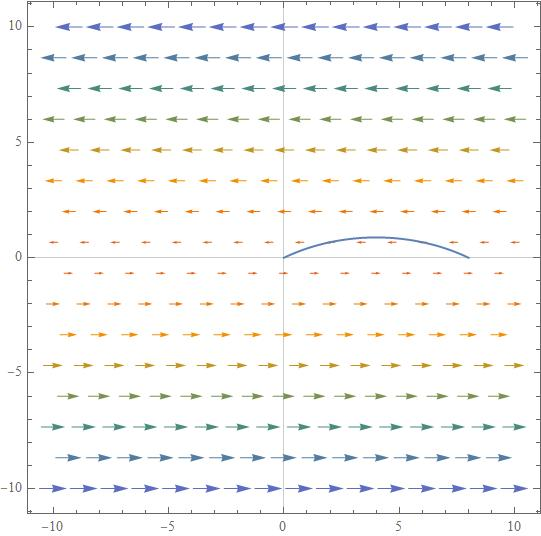
\includegraphics[width=0.9\textwidth]{lodka1}
		\captionof*{figure}{\textbf{Obrázek 1.} $x_0=8, y_0=0, V = 8,h=15$}
	\end{minipage}
	\begin{minipage}[b]{0.5\textwidth}
		\centering
		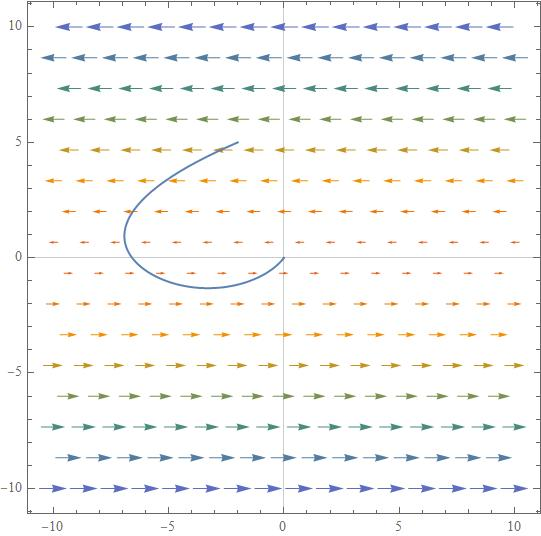
\includegraphics[width=0.9\textwidth]{lodka2}
		\captionof*{figure}{\textbf{Obrázek 2.} $x_0=-2, y_0=5, V = 2, h=15$}
	\end{minipage}
	\hfill
\end{minipage}
\subsection*{Počáteční podmínka $y_0=0$}
Všimněme si, že případ na obrázku (2) přejde pro $y=0$ na úlohu případu obrázku (1). Tento závěr není nijak překvapivý, protože pro tento model nepředpokládáme žádné zpoždění zatáčení a navíc její rychlost je čistě dána její polohou a parametry $V$ a $h$ (tedy v tomto systému nepředpokládáme žádné "nabrání" kinetické energie z předchozí části trajektorie). Rovněž není překvapivé, že pro $y_0=0$ je ideální trajektorie symetrická podle osy $x=\frac{x_0}{2}$. Toto tvrzení si nyní dokažme.\\
\\

Z informace $y_0=0$ a vztahu ~\eqref{eq:70} dostáváme
\begin{equation}
	\label{eq:75}
	\frac{1}{\cos\beta_{\navext, \navend}} = \frac{1}{\cos\beta_{\navext, \navstart}} \equiv  \cos\beta_{\navext, \navend} = \cos\beta_{\navext, \navstart}.
\end{equation}
Nyní využijme fyzikálního nadhledu. Jelikož se musíme dostat z počátečního bodu na ose $y=0$ do počátku, jistě musí platit
\begin{equation}
	\label{eq:76}
	\beta_{\navext, \navend}=-\beta_{\navext, \navstart}.
\end{equation}
Dále využijme toho, že $\tan x$ je lichá funkce. S tímto poznatkem a vztahy ~\eqref{eq:71}, ~\eqref{eq:76} dostáváme, že pro $t_{\navend, \navext}$ volbou $t_{\navstart}=0$ platí
\begin{equation*}
	\tan \beta_{\navext, \navstart} -  \tan \beta_{\navext, \navend} = -\tan \beta_{\navext, \navend} -  \tan \beta_{\navext, \navend}=-2\tan \beta_{\navext, \navend}
	=\frac{V}{h} (t_{\navstart} - t_{\navend, \navext})=-\frac{V}{h} t_{\navend, \navext} \implies
\end{equation*}
\begin{equation}
	\label{eq:77}
	t_{\navend, \navext}=\frac{2h}{V}\tan \beta_{\navext, \navend}.
\end{equation}
Opět využijme vztahu ~\eqref{eq:71} a vyjádřeme $\beta$ jako $\beta (t)$
\begin{equation*}
	\tan \beta_\navext = \frac{V}{h}(t-t_{\navend, \navext})+\tan \beta_{\navext, \navend}=\frac{V}{h}(t-\frac{2h}{V}\tan \beta_{\navext, \navend})+\tan \beta_{\navext, \navend}=\frac{V}{h}t - \tan \beta_{\navext, \navend} \implies
\end{equation*}
\begin{equation}
	\label{eq:78}
	\beta_\navext=\arctan\left( \frac{V}{h}t - \tan \beta_{\navext, \navend}\right) .
\end{equation}
V závěrečné fázi našeho dokazování si pomocí funkce $y(\beta_\navext)$, kterou si vyjádříme jako $y(t)$, ukážeme, že je symetrická podle času $\frac{t_{\navend, \navext}}{2}$, tedy že platí $y(\frac{t_{\navend, \navext}}{2}+\epsilon)=y(\frac{t_{\navend, \navext}}{2}-\epsilon)$.\\
Začněme vyjádřením $y=y(t)$ ze vztahu ~\eqref{eq:65}
\begin{equation}
	\label{eq:79}
	y(\beta_\navext(t))=h
	\left(
	\frac{1}{\cos \beta_{\navext}(t)}
	-
	\frac{1}{\cos \beta_{\navext, \navend}}
	\right)=h
	\left(
	\frac{1}{\cos \arctan(\frac{V}{h}t - \tan \beta_{\navext, \navend})}
	-
	\frac{1}{\cos \beta_{\navext, \navend}}
	\right)=
\end{equation}
\begin{equation*}
	=h
	\left(
	\frac{1}{\cos \arctan(\frac{V}{h}t - \tan \beta_{\navext, \navend})}
	-
	\frac{1}{\cos \beta_{\navext, \navend}}
	\right)=h\left(
	\sqrt{\left( \frac{V}{h}t-\tan \beta_{\navext, \navend}\right)^2 + 1 }
	-
	\frac{1}{\cos \beta_{\navext, \navend}}
	\right) \implies
\end{equation*}
\begin{equation}
	\label{eq:80}
	y(t)=h\left(
	\sqrt{\left( \frac{V}{h}t-\tan \beta_{\navext, \navend}\right)^2 + 1 }
	-
	\frac{1}{\cos \beta_{\navext, \navend}}
	\right).
\end{equation}
Ve výpočtu se nám objevila zajímavá identita $\cos \arctan$, pro kterou platí $\cos \arctan (x)=\frac{1}{\sqrt{x^2+1}}$. Nyní nám už zbývá dosadit hodnotu $t = \frac{ t_{\navend, \navext}}{2}\pm\epsilon$ do $y(t)$.
\begin{equation*}
	y\left( \frac{ t_{\navend, \navext}}{2}\pm\epsilon\right) =h\left(
	\sqrt{\left( \frac{V}{h}\left( \frac{ t_{\navend, \navext}}{2}\pm\epsilon\right) -\tan \beta_{\navext, \navend}\right)^2 + 1 }
	-
	\frac{1}{\cos \beta_{\navext, \navend}}
	\right)=
\end{equation*}
\begin{equation*}
	=h\left(
	\sqrt{\left( \frac{V}{h}\left( \frac{\frac{2h}{V}\tan\beta_{\navext, \navend}}{2}\pm\epsilon\right) -\tan \beta_{\navext, \navend}\right)^2 + 1 }
	-
	\frac{1}{\cos \beta_{\navext, \navend}}
	\right)=
\end{equation*}
\begin{equation}
	\label{eq:81}
	=h\left(
	\sqrt{\left( \tan \beta_{\navext, \navend}\pm\epsilon -\tan \beta_{\navext, \navend}\right)^2 + 1 }
	-
	\frac{1}{\cos \beta_{\navext, \navend}}
	\right)=h\left(\sqrt{\epsilon^2+1}-\frac{1}{\cos \beta_{\navext, \navend}}
	\right)
\end{equation}
Tedy jsme ukázali, že řešení se pohybuje symetricky podle času $t=\frac{ t_{\navend, \navext}}{2}$. To ovšem nedává tvrzení, jelikož nevíme, jak se řešení chová pro $x$-ovou souřadnici. Ta je ovšem analyticky složitá na řešení, avšak máme jiný způsob, jak získat dodatečnou informaci a to pomocí okamžitého natočení $\beta_{\navext}(t)$, kterou jsme si při výpočtu odvodili.\\
Aby naše tvrzení bylo dokázáno musíme ukázat, že platí $\beta_{\navext}(\frac{ t_{\navend, \navext}}{2}+\epsilon)=-\beta_{\navext}(\frac{ t_{\navend, \navext}}{2}-\epsilon)$. To již není žádný problém, jelikož platí
\begin{equation*}
	\beta_{\navext}\left( \frac{ t_{\navend, \navext}}{2}\pm\epsilon\right) =\arctan\left( \frac{V}{h}\left( \frac{ \frac{2h}{V}\tan\beta_{\navext, \navend}}{2}\pm\epsilon\right) - \tan \beta_{\navext, \navend}\right) 
	= \arctan\left( \tan \beta_{\navext, \navend}\pm\epsilon - \tan \beta_{\navext, \navend}\right)
	=\arctan(\pm\epsilon)
\end{equation*}
\begin{equation}
	\label{eq:82}
	\implies \beta_{\navext}\left( \frac{ t_{\navend, \navext}}{2}\pm\epsilon\right) =\pm\arctan(\epsilon).
\end{equation}
Tedy z ~\eqref{eq:82} vidíme, že natočení je rovněž symetrické podle času $t=\frac{ t_{\navend, \navext}}{2}$ (přesněji řečeno lichá vzhledem k tomuto času). S touto a ještě informací o závislosti $y$-ové složky (která je naopak sudá vzhledem k tomuto času) dostáváme tvrzení. $\qed$

\end{document}
